 
\documentclass[10pt]{article}

\usepackage[slovak]{babel}
\usepackage[utf8]{inputenc}
\usepackage[T1]{fontenc}
\usepackage{graphicx}

\usepackage{times}


\usepackage[margin=1in]{geometry} 
\usepackage{amsmath,amsthm,amssymb}
 
\newcommand{\N}{\mathbb{N}}
\newcommand{\Z}{\mathbb{Z}}
 
\newenvironment{theorem}[2][Theorem]{\begin{trivlist}
\item[\hskip \labelsep {\bfseries #1}\hskip \labelsep {\bfseries #2.}]}{\end{trivlist}}
\newenvironment{lemma}[2][Lemma]{\begin{trivlist}
\item[\hskip \labelsep {\bfseries #1}\hskip \labelsep {\bfseries #2.}]}{\end{trivlist}}
\newenvironment{exercise}[2][Exercise]{\begin{trivlist}
\item[\hskip \labelsep {\bfseries #1}\hskip \labelsep {\bfseries #2.}]}{\end{trivlist}}
\newenvironment{reflection}[2][Reflection]{\begin{trivlist}
\item[\hskip \labelsep {\bfseries #1}\hskip \labelsep {\bfseries #2.}]}{\end{trivlist}}
\newenvironment{proposition}[2][Proposition]{\begin{trivlist}
\item[\hskip \labelsep {\bfseries #1}\hskip \labelsep {\bfseries #2.}]}{\end{trivlist}}
\newenvironment{corollary}[2][Corollary]{\begin{trivlist}
\item[\hskip \labelsep {\bfseries #1}\hskip \labelsep {\bfseries #2.}]}{\end{trivlist}}
 
\begin{document}
 
% --------------------------------------------------------------
%                         Start here
% --------------------------------------------------------------
 
%\renewcommand{\qedsymbol}{\filledbox}
 
\title{TIN - Domáca úloha č. 3}%replace X with the appropriate number
\author{Roman Dobiáš - xdobia11@stud.fit.vutbr.cz}
 
\maketitle

\section*{Úloha č.1}
\subsection*{Identifikácia funkcie}
Zjavne sa jedná o \textit{Fibbonaciho postupnosť}. Páska č. 1 indikuje číslo N v zápise 1tiek, pre ktoré je funkcia Fib vypočítaná. Pásky 2 a 3 sľúžia na uchovanie predchádzajúcich dvoch
hodnôt postupnosti. 

Fibonačiho postupnosť je možné matematicky zadefinovať nasledujúco:
\begin{align}
    Fib(n) = 
    \begin{cases}
        0 & n = 0\\
        Fib(n-1) & n = 1\\
        Fib(n-1)\times Fib(n-2) & inak
    \end{cases}
\end{align}
\subsection*{Vyjadrenie funkcie pomocou primitívnej rekurzie}

Jedným z riešení je zaviesť pomocnú funkciu $K(x)$, ktorej vyčíslenie bude zodpovedať dvojici $(F(x), F(x+1)$ kde $F$ bude funkcia Fibbonaci.

Funkciu $K$ definujeme pomocou primitívnej rekurzie nasledujúco:

\begin{align*}
    K(0) &= \xi \times ( \sigma  \mathbin{o} \xi ) () \\
    K(x+1) &= \pi_3^3 \times (plus  \mathbin{o} ( \pi_2^3 \times \pi_3^3)  (x, K(x))
\end{align*}

Výsledná funkcia $F(x)$ má potom tvar:

\begin{align*}
    F(x) = (\pi_2^2 \mathbin{o} K) (x)
\end{align*}

\section*{Úloha č.2}
Diagonalizáciou ukážeme, že počet ohodnotení unárneho predikátu \textit{u} nad spočetným univerzom je nespočetný. Počet ohodnotení predikátu je totiž rovný $2^{\mathbb{N}}$, pretože pre každý prvok x z $\mathbb{N}$ prvkov univerza môžeme definovať $p(x)$ alebo $\neg p(x)$.

\begin{proof}
    Predpokladajme, že počet realizácii je spočetný. Potom existuje zobrazenie $f: \mathbb{N} \to$ 
    Uvažujme nekonečnú maticu
\end{proof}
\section*{Úloha č.3}

\begin{proof}
$\mathcal{O}(3^{2n}) \subseteq \mathcal{O}(2^{3n})$ \\
Z definície pre každú funkciu $f \in \mathcal{O}(3^{2n})$ platí, že $\exists c \in \mathbb{R}: \exists n_0 \in \mathbb{N}: \forall n > n_0: f(n) \leq c\times 3^{2n}$.  
Na to, aby $\mathcal{O}(3^{2n}) \subseteq \mathcal{O}(2^{3n})$ stačí ukázať, že každá funkcia $f \in \mathcal{O}(3^{2n})$ je ohraničená v $\mathcal{O}(2^{3n})$.

Predpokladajme, že platí práve spomenutý vzťah. Potom pre každú funkciu $f$ platí, že $\exists c,d \in \mathcal{R}^+: c \times 3^{2n} \leq d \times 2^{3n}$. 

Potom ale platia nasledujúce úpravy:

\begin{align*}
    c \times 3^{2n} \leq d \times 2^{3n}  \\
    1 \leq \frac{d \times 2^{3n}}{c \times 3^{2n}} \\
    1 \leq \frac{d}{c} \times \frac{2^{3n}}{3^{2n}} \\
    1 \leq \frac{d}{c} \times (\frac{2^{3}}{3^{2}})^n \\
    1 \leq \frac{d}{c} \times (\frac{8}{9})^n \\
\end{align*}
Platí, že $\lim_{n \to \infty} (\frac{8}{9})^n = 0$, teda platí, že $\lim_{n \to \infty} 1 \leq \frac{d}{c} \times (\frac{8}{9})^n  = 1 < 0$, čo je spor.
Preto neplatí $\mathcal{O}(3^{2n}) \subseteq \mathcal{O}(2^{3n})$.
\end{proof}

\begin{proof}
$\mathcal{O}(2^{3n}) \subseteq \mathcal{O}(3^{2n})$ \\
Z definície pre každú funkciu $f \in \mathcal{O}(2^{3n})$ platí, že $\exists c \in \mathbb{R}: \exists n_0 \in \mathbb{N}: \forall n > n_0: f(n) \leq c\times 2^{3n}$.  
Na to, aby $\mathcal{O}(2^{3n}) \subseteq \mathcal{O}(3^{2n})$ stačí ukázať, že každá funkcia $f \in \mathcal{O}(2^{3n})$ je ohraničená v $\mathcal{O}(3^{2n})$.

Predpokladajme, že platí práve spomenutý vzťah. Potom pre každú funkciu $f$ platí, že $\exists c,d \in \mathcal{R}^+: c \times 2^{3n} \leq d \times 3^{2n}$. 

Potom ale platia nasledujúce úpravy:

\begin{align*}
    c \times 2^{3n} \leq d \times 3^{2n}  \\
    1 \leq \frac{d \times 3^{2n}}{c \times 2^{3n}} \\
    1 \leq \frac{d}{c} \times \frac{3^{2n}}{2^{3n}} \\
    1 \leq \frac{d}{c} \times (\frac{3^{2}}{2^{3}})^n \\
    1 \leq \frac{d}{c} \times (\frac{9}{8})^n \\
\end{align*}
Ak zvolíme $d = c$, potom už pre $n = 0$ platí, že $1 \leq (\frac{9}{8})^n$.
Ukázali sme teda, že pre každú $f \in \mathcal{O}(2^{3n})$ sme schopný nájsť danú konštantu $d$ tak, aby $f$ bola ohraničená funkciou $\mathcal{O}(3^{2n})$.
Platí teda $\forall f \in \mathcal{O}(2^{3n}): f \in \mathcal{O}(3^{2n})$, teda platí $\mathcal{O}(2^{3n}) \subseteq \mathcal{O}(3^{2n})$. 
\end{proof}

\section*{Úloha č.4}
Rozhodovací problém farbenia grafov je jazyk ColorGraph = $\{$ (<V>,<E>\#k) | G = (<V>, <E>) je graf
ofarbitelný k farbami \}.
Redukcia z farbenia grafov na problem tedy Kvety 
\subsection*{Algoritmus prevodu}
Každú inštanciu jazyka ColorGraph sme schopný previesť na problém Tety Kvety nasledujúci:
\begin{itemize}
    \item Pre každý uzol E vygenerujeme K+1 surovín, kde každá surovina má kapacitu 1 (teda, Teda
        Kveta má práve 1 túto surovinu). K surovín reprezentuje jednotlivé z K farieb a K+1 surovina
        je použitá pre detekovanie, či už je vrchol ofarbený.
        Jednotlivé z K+1 surovín označme ako $E_i, 0 \leq i < k$.
    \item Pre každé ofarbenie uzla E farbou F 
    \begin{itemize}
        \item vypočítame množinu vrcholov I takých, že existuje hrana medzi vrcholom E a vrcholom z
            I a prizjednotíme vrchoľ E
        \item vytvoríme "pečivo" $E_F$, ktorého ingrediencie sú suroviny $a_i, a \in I, i = F$ a
            surovina $E_F$.
    \end{itemize}
    \item Pre takto zakódovaný problém riešime problém Tety Kvety pre počet priateľok $k$, kde $k = |V|$.
    \item Graf je ofarbiteľný práve vtedy, ak môžeme každý vrchol ofarbiť farbou tak, že
        priliehajúce vrcholy nemaju tú istú farbu.
    \item Zrejme platí, že ak upečiem pečivo $E_F$, potom toto pečivo bude pre daný vrchol jediné
        (vďaka surovine K+1) a zároveň priliehajúce vrcholy nebudú mať rovnaké pečivo (farbu),
        pretože surovina ich farby už bola vyčerpaná pri pečení $E_F$.
    \item Teda platí, že ak je možné upiecť N rôznych pečív, kde N je počet vrcholov a zároveň
        platia tézy vyššie, potom graf je K-ofarbiteľný.
\end{itemize}
\subsection*{Príklad}
Uvažujme graf A-B, B-C, C-D, D-A. 
Reprezentáciu úlohy môžeme vyjadriť tabulkou:
TODO
suroviny ako hlavička, pečio ako riadky, Y osa ako vybrané pečivá
\section*{Úloha č.5}
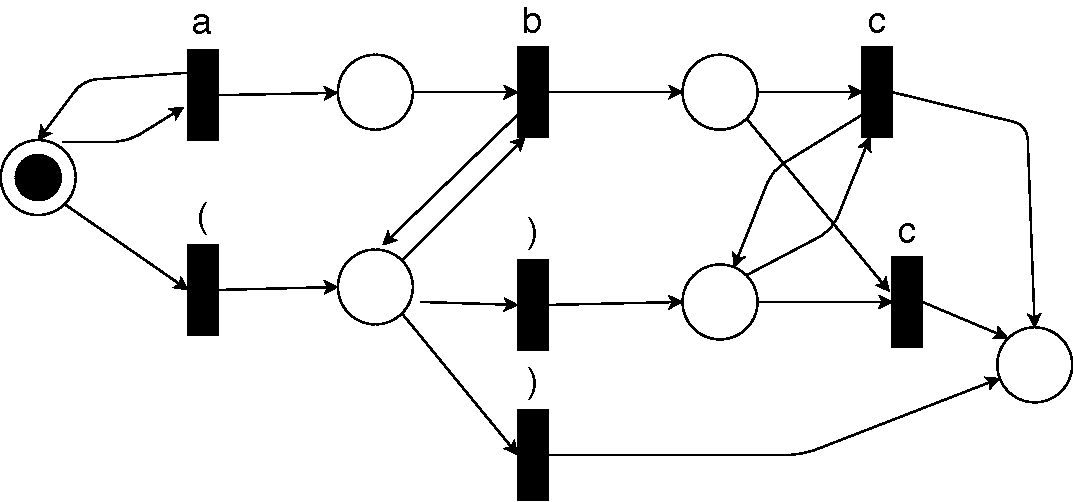
\includegraphics{petriNetFinalTake.pdf}



\end{document}
